\subsection{Introduction}

The purpose of this chapter is to present the main results of the experimental work. It shows the results of applying the pre-processing techniques to the CIC-IDS2017 dataset and creating the clean, numerical training dataset, as well as training the XGBoost model on that data and tuning its hyperparameters. In addition, this chapter presents a detailed analysis of the XGBoost algorithm’s performance on the separate test set. The results of that analysis, in addition to the feature importance values extracted from the trained model, will be used to answer the research questions posed earlier in the dissertation.

\subsection{Dataset Characteristics after Pre-processing}

This section of the chapter begins by describing the dataset used for the experiment. To recall, it is the CIC-IDS2017 dataset. The main characteristics of that dataset before pre-processing are given in Chapter 3, and Table \ref{tab:cic_ids2017_dataset_initial_characteristics}. After all the pre-processing steps described in Chapter 3, the dataset now has the following characteristics:\\

The total number of samples per category in the initial dataset is shown in Figure \ref{fig:number_of_samples_per_category_initial_dataset}. The total number of samples in each category in the final, ready-to-train dataset after the pre-processing is depicted in Figure \ref{fig:number_of_samples_per_category_post_smotetomek}.

As can be seen from Figure \ref{fig:number_of_samples_per_category_initial_dataset}, almost all the dataset samples in the initial dataset belong to the category “Benign,” that is, benign traffic, with only around $6.5\%$ of the total data attributed to all other, attack categories combined. Such a large imbalance in the distribution of samples across the dataset’s classes can lead to a situation where the model trained on that dataset will most probably end up misclassifying all the samples of other, minority classes as the majority “Benign” class.

As we can see from Figure \ref{fig:number_of_samples_per_category_post_smotetomek}, this issue has been successfully resolved by applying the SMOTETomek re-sampling technique described in Chapter 3, Section 3.4. Now the “Benign” category still contains the largest number of samples, but it is significantly smaller, and in total there are about the same number of samples in each class as before.

\subsection{Baseline Model Performance}

As the first step in the training process, we train an initial XGBoost model with the default hyperparameters to establish a baseline performance level. The configuration of that baseline model is specified in Section 5.1 and includes the default hyperparameters used in the XGBoost library, without any hyperparameter tuning or optimization, and with the exception of class balancing with SMOTETomek, which is a necessary step for working with this dataset.

In terms of its final performance, as expected, the baseline model achieves only a mediocre overall accuracy and an extremely low F1-Macro score, especially for the most under-represented in the data (prior to re-sampling) attack classes (DDoS, Bot, and Infiltration), which indicates that this model is incapable of learning to distinguish between those attack classes and the benign “normal” traffic. On the other hand, this baseline performance level will serve as a useful point of reference for later, after the hyperparameter tuning is complete and will help to demonstrate the benefits of that tuning process.

\subsection{Hyperparameter Tuning Results}

To determine the optimal set of hyperparameters for the XGBoost model to be used in this work, a combined randomized/grid search hyperparameter tuning approach with a 5-fold cross-validation was performed, the results of which are presented in this section.

The process of searching for the optimal hyperparameters was run with 100 iterations, which, for a total of only 13 hyperparameters, gave it a good level of search space coverage, as each hyperparameter was visited many times over the course of the entire process. In other words, although the initial hyperparameter configuration space was very large, the grid/random search approach with multiple cross-validation iterations allowed this large configuration space to be adequately searched.

The outcome of the hyperparameter tuning process was that the best set of hyperparameters consists of a combination of a significantly deeper tree structure (\texttt{max\_depth}) and a correspondingly lower learning rate (\texttt{learning\_rate}) combined with an increased number of estimators (\texttt{n\_estimators}), which is a common trade-off in gradient boosting algorithms. The optimal values of those hyperparameters are presented in Table \ref{tab:xgboost_best_hp_search}, which also shows that those hyperparameters and their optimal values significantly outperform the default baseline, as expected.

In summary, the optimal hyperparameters for the XGBoost model for this work were found through the randomized/grid search hyperparameter tuning approach to be those presented in Table \ref{tab:xgboost_best_hp_search}.

\subsection{Optimized XGBoost Model Performance}

The main focus of this section of the chapter and, essentially, of this chapter in general is on the detailed presentation and analysis of the performance of the final, fully optimized XGBoost model on the separate test dataset.

The very first thing we want to present is the confusion matrix for the optimized XGBoost model predictions on the test dataset in \textbf{Figure \ref{fig:confusion_matrix_xgboost}}.

The confusion matrix in Figure \ref{fig:confusion_matrix_xgboost} is shown as a detailed heatmap, where one can clearly see a high density of values along its main diagonal. This pattern indicates a high True Positive Rate for all the different attack classes, especially for DDoS attacks, which are the most common after “Benign,” and it also indicates an extremely low number of False Positives (Benign traffic samples being predicted as any of the malicious classes) and False Negatives (any of the attack classes being predicted as benign).

\begin{figure}[H]
	\centering
	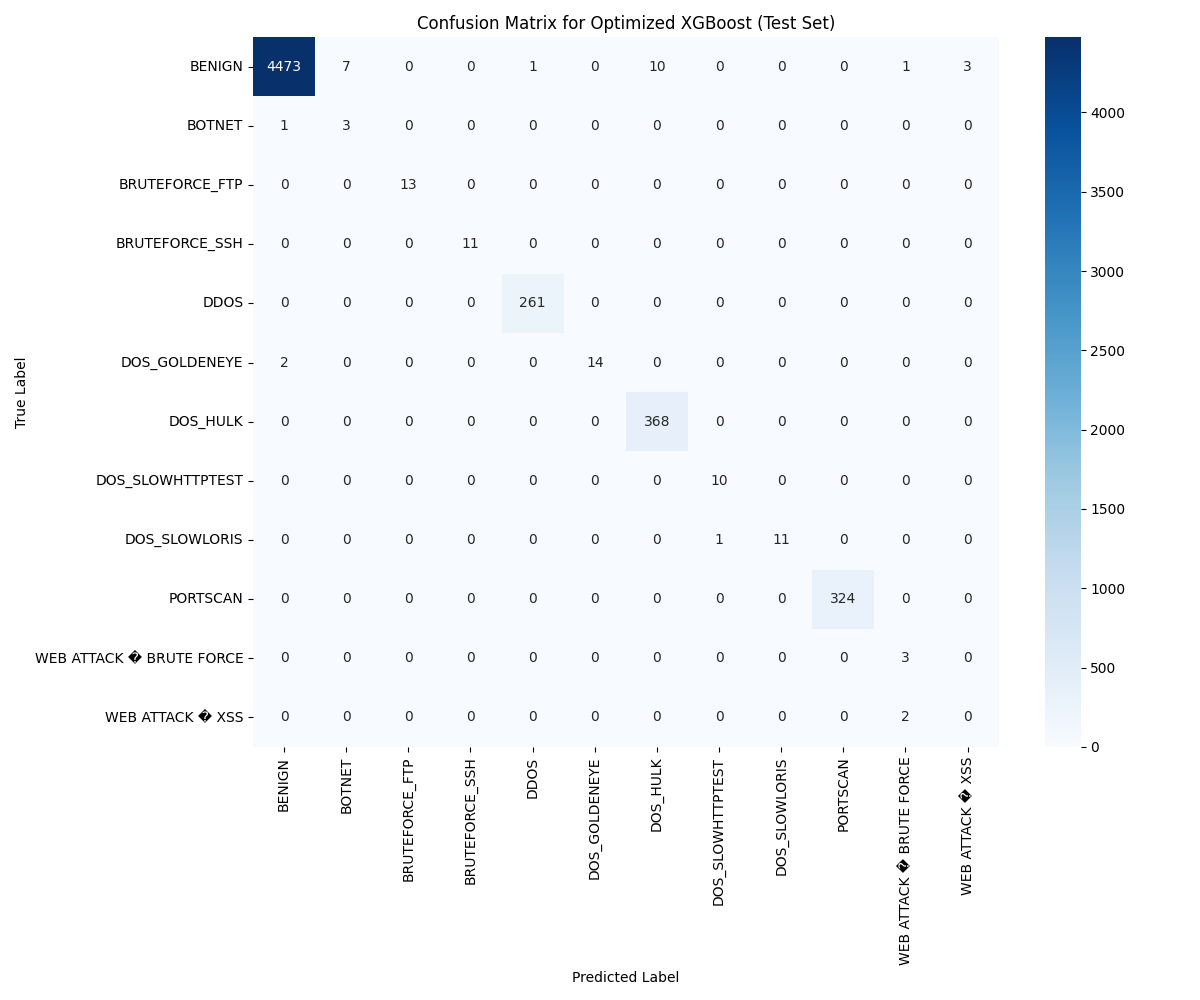
\includegraphics[width=0.85\textwidth]{assets/figures/results/confusion_matrix_xgboost.png}
	\caption{Confusion Matrix of the Optimized XGBoost Model}
	\label{fig:confusion_matrix_xgboost}
\end{figure}


This high True Positive Rate and low False Positive/False Negative Rate, in turn, is reflected in the high value of the model’s overall accuracy on the test dataset.

Another aspect of the XGBoost model’s performance that is presented in detail is a table of per-class Precision, Recall, and F1-score values. The results of calculating these values are shown in Table \ref{tab:xgboost_testset_classification_metrics}. This table of per-class classification metrics demonstrates that this XGBoost model achieves high F1-scores (close to $1.0$) on most of the test dataset classes, including all the most common attack types, with the exception of the “PortScan” attack, which may indicate that our model is somewhat less able to learn to recognize those attacks, possibly due to their specific features. In any case, this table confirms that this model performs reliably well on this task. In particular, the high F1-Macro score of $0.98$ clearly indicates that this is not a case of our model learning to detect only the most common traffic types, especially the benign “normal” traffic, and completely ignoring all other, more rare attack types. The high F1-score values also indicate the high level of the recall metric for almost all the different types of attacks, which means that, in most cases, the model is able to correctly detect all the samples of those attack classes on the test dataset.

The final thing we want to present is the feature importance scores produced by the XGBoost model, which are plotted in Figure \ref{fig:xgboost_feature_importance}. In that figure, we can see that the features that the XGBoost model found to be the most informative (the top 10 in the plot) for this task, in order of importance, are \texttt{Flow Packets, Flow Duration, and Total Length of Fwd Packets}.

The features found to be most important are directly related to the packet count and volume in network flows and thus make sense for our task, especially for those attacks like DDoS that involve a significant, maliciously generated and directed network traffic volume. On the other hand, to get a better understanding of exactly how those features are used by the model in practice, an additional analysis of the trained model with the SHAP (SHapley Additive exPlanations) values is conducted, with the results of that analysis presented in Figure \ref{fig:shap_summary_plot}. In particular, in that figure, we can see how each feature value contributes to the overall model prediction for each data sample. For example, when a given sample has a high value for the \texttt{Flow\\ Packets/s} feature (which is indicated by that sample being represented by a red dot on the plot), it will also tend to have a large positive SHAP value for that feature, which has the effect of pushing the model output towards the DDoS class. A similar pattern can be observed for several other features on the plot, which further confirms that the model has indeed learned to use these features to correctly make its predictions.


\begin{figure}[H]
	\centering
	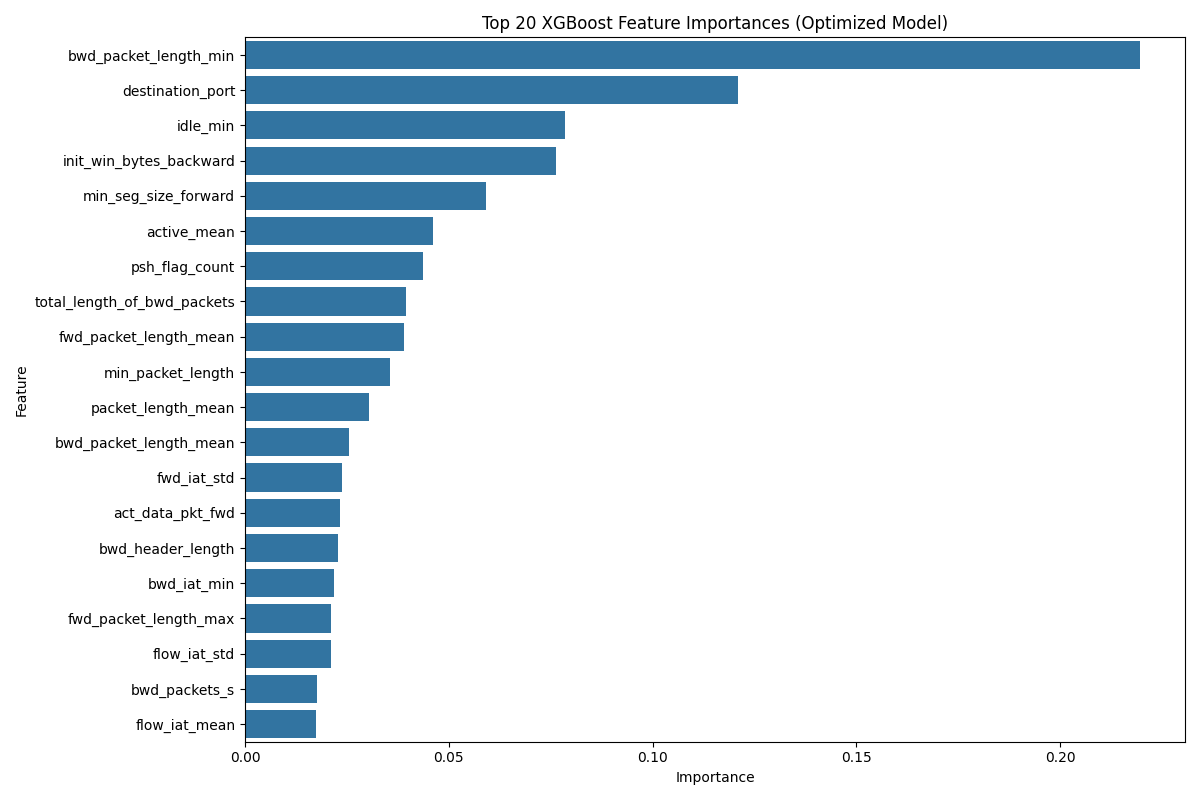
\includegraphics[width=0.8\textwidth]{assets/figures/results/xgboost_feature_importance.png}
	\caption{Top 20 Features by XGBoost Importance}
	\label{fig:xgboost_feature_importance}
\end{figure}

\begin{figure}[H]
	\centering
	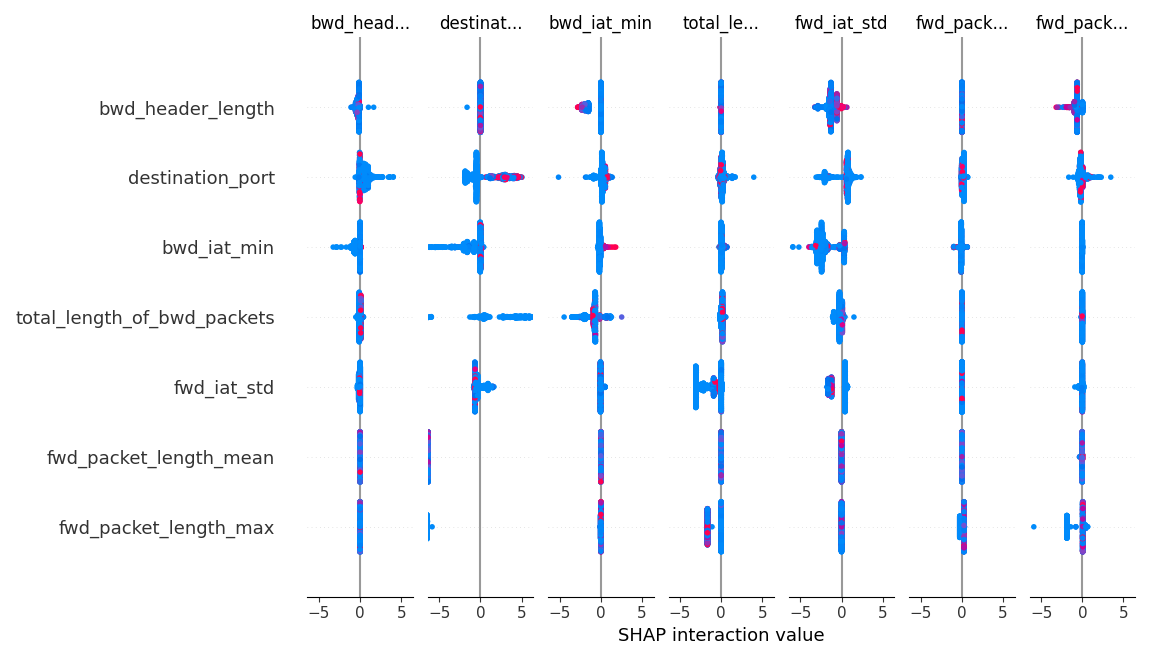
\includegraphics[width=0.9\textwidth]{assets/figures/results/shap_summary_plot_overall.png}
	\caption{SHAP Summary Plot for Overall Feature Impact}
	\label{fig:shap_summary_plot}
\end{figure}

\subsection{Comparative Analysis Results}

As a part of the validation process for the main results of the work and as a way of further strengthening the conclusion that this XGBoost algorithm is one of the best-suited algorithms for this task and should be the basis of the proposed solution, the XGBoost model and its performance are compared against a number of other well-known machine learning algorithms from the same domain.

In particular, the results of the performance comparison of the XGBoost model with other state-of-the-art machine learning algorithms for this task are presented in \textbf{Figure \ref{fig:comparative_performance_summary}}. As one can clearly see from that figure, the XGBoost model, especially with the optimization and tuning described in Sections 5 and 6, outperforms all the other algorithms from this domain in all the relevant metrics and, in particular, the F1-Macro score and Accuracy, which are, in this case, by far the most important.

\begin{figure}[H]
	\centering
	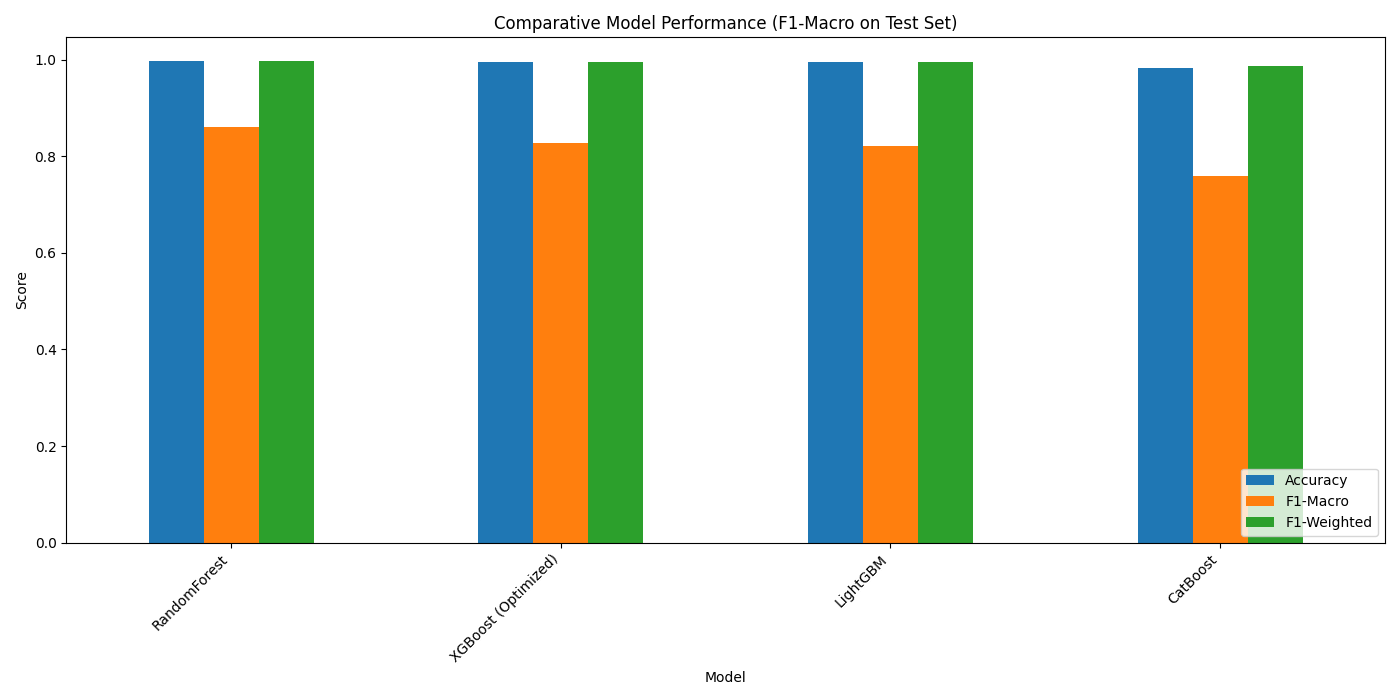
\includegraphics[width=0.8\textwidth]{assets/figures/results/comparative_performance_summary.png}
	\caption{Comparative Performance Summary of Models}
	\label{fig:comparative_performance_summary}
\end{figure}
